\setcounter{chapter}{2}
\chapter{Cross section calculation}
\label{Sect:cr_sect}


\section{$W$-smearing and boundary blurring of the $Q^{2}$ versus $W$ distribution}
\label{Sect:smearing_blurring}

The smearing of the invariant mass $W$ has the same origin as the smearing of the missing mass, which is already discussed in Sect.~\ref{Sect:excl_cut}, but since $W$ is the variable needed to describe the reaction (and the extracted cross section is binned in $W$), the issue of $W$-smearing requires special attention and, therefore, is separately addressed here.


For the process of double-pion electroproduction off the proton (as for any other exclusive process) the reaction's invariant mass can in general be determined in two ways, i.e. either from the initial particle  four-momenta\footnote[1]{Although the scattered electron is treated as a final particle, here it is classified as ``initial", since it defines the virtual photon, which in turn is attributed to the initial state.} ($W_{i}$) or from the final particle  four-momenta ($W_{f}$) as Eqs.~\eqref{W_fin_1} and~\eqref{W_fin_2} demonstrate. 


%\begin{equation}
\begin{eqnarray}
W_{i}&= & \sqrt{(P_{p}^{\mu}+P_{\gamma_{v}}^{\mu})^{2}} \label{W_fin_1} \\
W_{f}&= & \sqrt{(P_{\pi^{+}}^{\mu}+P_{\pi^{-}}^{\mu}+P_{p'}^{\mu})^{2}} \label{W_fin_2}
\end{eqnarray}
%\end{equation}

Here $P_{\pi^{+}}^{\mu}$, $P_{\pi^{-}}^{\mu}$, and $P_{p'}^{\mu}$ are the four-momenta of the final state hadrons, $P_{p}^{\mu}$ is the four-momentum of the initial proton and $P_{\gamma_{v}}^{\mu}=P_{e}^{\mu}-P_{e'}^{\mu}$ the four-momentum of the virtual photon with $P_{e}^{\mu}$ and $P_{e'}^{\mu}$ the four-momenta of the incoming and scattered electrons, respectively. 

To determine $W_{f}$, all final hadrons should be registered, while for the calculation of $W_{i}$ it is sufficient to register the scattered electron. The latter opportunity allows event samples with one unregistered final hadron, whose four-momentum is recovered via the missing mass technique, to be used. This approach allows for a significant increase of the analyzed statistics (see Sect.~\ref{Sect:excl_cut}).

In experiments off protons at rest $W_{f}$ and $W_{i}$ may differ due to the detector resolution and the radiative effects, which electrons undergo. In moving proton experiments one more aspect takes effect, i.e. in order to calculate $W_{i}$, one needs information about the target proton momentum ($P_{p}^{\mu}$), which is accessible only in the fully exclusive topology\footnote[2]{If the spectator nucleon momentum is not directly measured in the experiment. This was not an option in the analyzed ``e1e" experiment. }. Therefore, the value of  $W_{i}$ given by Eq.~\eqref{W_fin_1} turns out to be ill-defined, if one of the final hadrons is not registered. This brings us to the choice to either demand the registration of all final hadrons to determine $W_{f}$ (that reduces the flexibility of the analysis) or to work under a so-called ``target-at-rest-assumption", which assumes the initial proton to be at rest. In the last approach the value of $W_{i}$ appears to be smeared. This smeared value of the invariant mass is hereinafter denoted as $W_{sm}$. Meanwhile, the value $W_{f}$ corresponds to the true reaction invariant mass and, therefore, is denoted as $W_{true}$. It can be calculated only in the fully exclusive topology.

If a smeared value $W_{sm}$ is used to describe the reaction, the extracted cross sections turned out to be convoluted with a function that is determined by the Fermi motion of the initial proton~\cite{Skorodumina:2015rea,twopeg-d}. To retrieve the non-smeared observable, a correction that unfolds this effect should be applied to the cross sections.


Beside the $W$-smearing, the Fermi motion of the target proton is also responsible for the boundary blurring of the $Q^{2}$ versus $W$ distribution\footnote[3]{This issue is addressed in more details in Ref.~\cite{twopeg-d}.}. This happens because the experiment off the moving proton with fixed laboratory beam energy is equivalent to that off the proton at rest performed with altered effective beam energy~\cite{twopeg-d}. The boundaries of the $Q^{2}$ versus $W$ distribution, however, are beam energy dependent. Therefore, the distribution edges, being sharp and distinct in the proton at rest experiment, become blurred in the experiment off a moving proton.


The blurring, however, affects only the edges of $Q^{2}$ versus $W_{true}$ distribution, where $W_{true}$ is the true reaction invariant mass given by Eq.~\eqref{W_fin_2}, since $W_{true}$ accounts for the target motion and, therefore, for the alteration of the effective beam energy. If the smeared value $W_{sm}$, calculated by Eq.~\eqref{W_fin_1} under the target-at-rest-assumption, is used instead, the distribution edges are not subject to the blurring because the fixed value of the laboratory beam energy is used in calculations.

\begin{figure}[htp]
\begin{center}
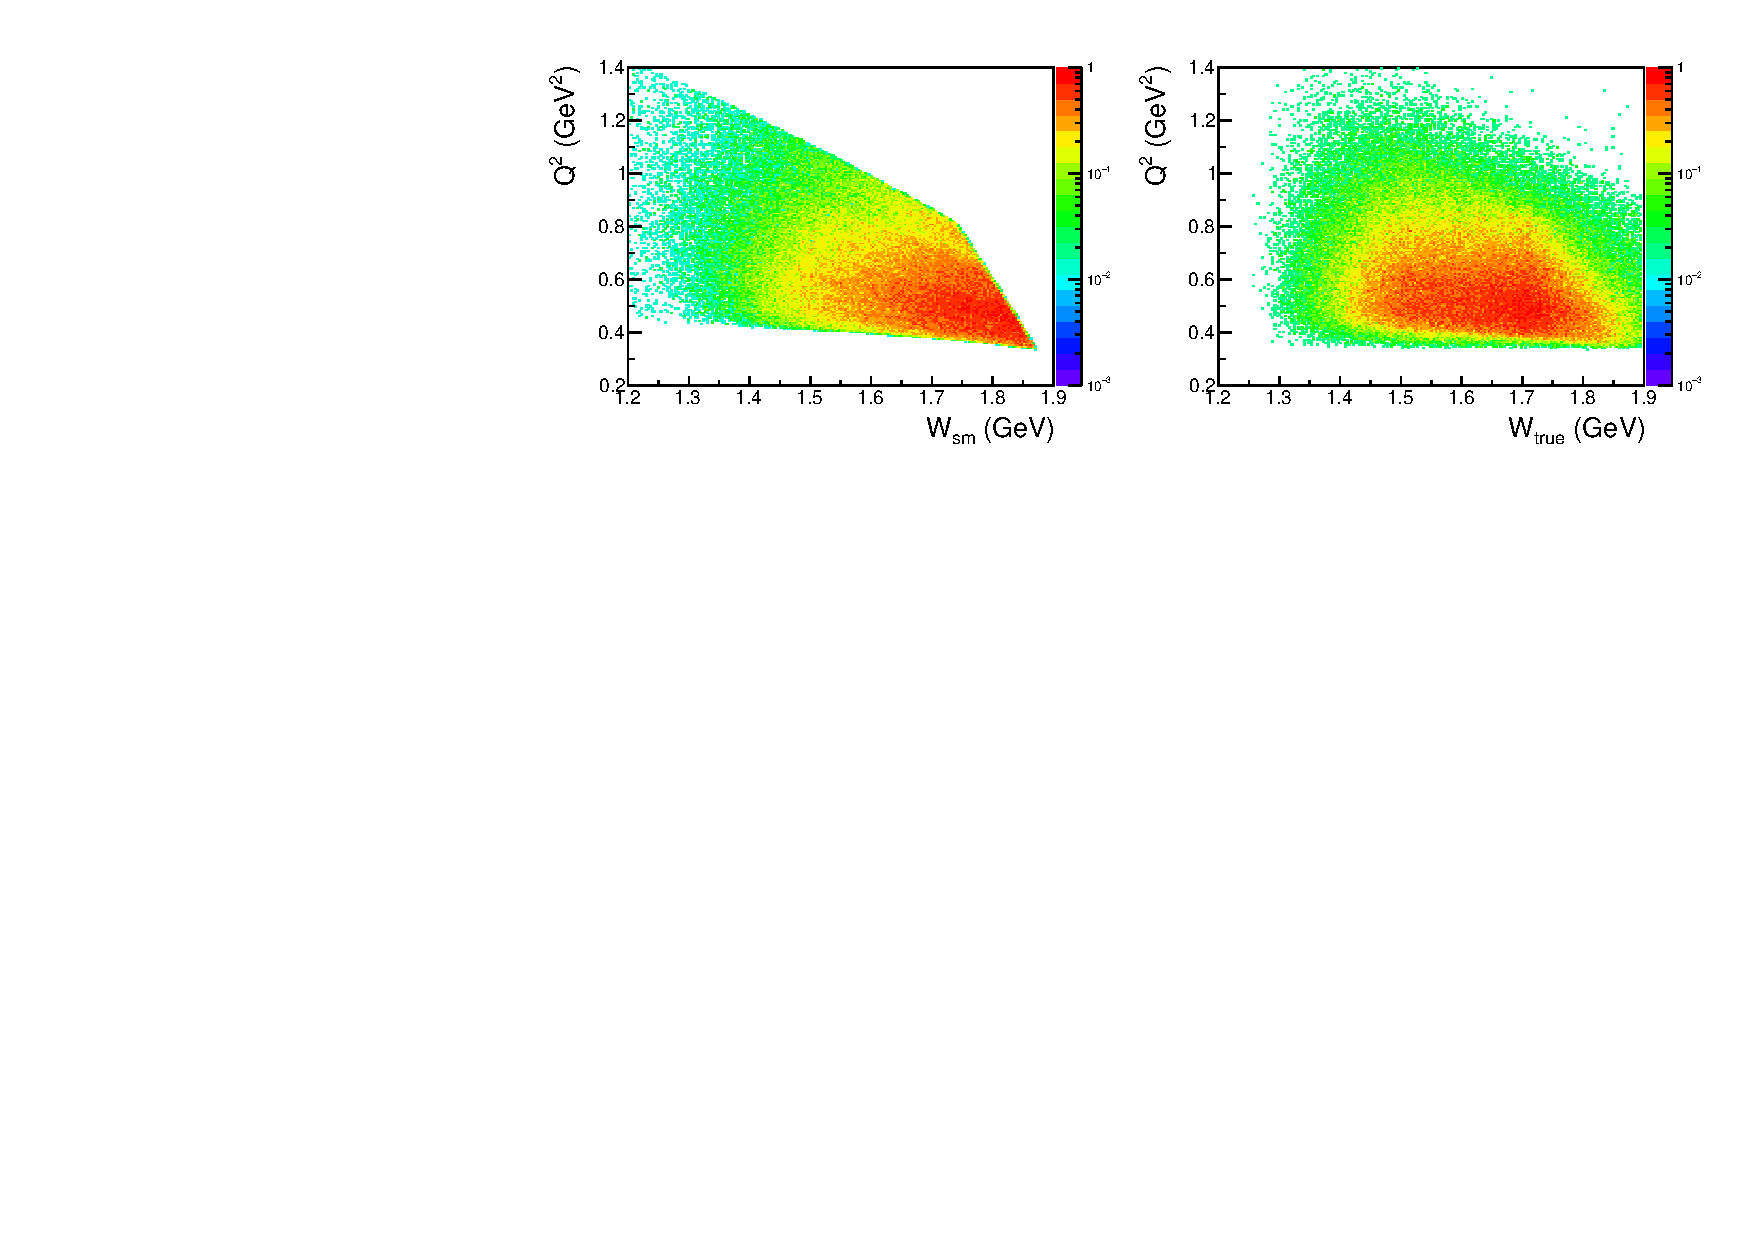
\includegraphics[width=16.5cm]{pictures/cross_section/blurring.pdf}
\caption{\small Experimental $Q^2$ versus $W$ distributions for $W_{sm}$ (left) and $W_{true}$ (right) plotted for the fully exclusive topology. The boundaries of the left distribution are sharp, since the $W_{sm}$ is calculated under the target-at-rest-assumption and the fixed value of the laboratory beam energy is used in calculations. The boundaries of the right distribution are blurred, since the calculation of $W_{true}$ accounts for the target proton motion and therefore for the alteration of the effective beam energy of the experiment.} \label{fig:blurring}
\end{center}
\end{figure}

This situation is illustrated in Fig.~\ref{fig:blurring}, where the $Q^2$ versus $W$ distributions are shown for $W_{sm}$ (left) and $W_{true}$ (right). These distributions are plotted for the fully exclusive topology only, since it allows for the determination of both $W_{sm}$ and $W_{true}$. The distributions, therefore, contain only a small portion of the total analyzed statistics. The boundaries of the left distribution are sharp, since the $W_{sm}$ is calculated assuming the fixed laboratory beam energy and the target at rest. The boundaries of the right distribution are blurred, since the calculation of $W_{true}$ accounts for the target proton motion and, therefore, for the alteration of the effective beam energy of the experiment.


The event yield in the blurred region suffers from depletion of events (compared to that for the case of fixed beam energy and sharp distribution edges). To estimate this effect, one should know the function that describes the alteration of the effective beam energy. This function is in turn determined by the target proton momentum distribution. The cross sections extracted in the blurred region need a special correction, otherwise they will suffer from the underestimation.


The situation described above offers two options, i.e. to use either $W_{sm}$ or $W_{true}$ to describe the reaction. The former opportunity leads to the need to apply a correction that unfolds the cross section smearing, while the latter requires the correction due to the blurring effect. The first option was chosen in this analysis because it has the advantage of using the $\pi^{-}$ missing topology that accumulates the majority of the experimentally available statistics. 

Thus, to calculate the cross section in this analysis, events are binned in $W_{sm}$. Note, however, that the corresponding $W$ points on the chosen $W_{sm}$ grid (see Sect.~\ref{Sect:binning}) are then treated as actual $W$-values where the cross section is eventually reported. However, the cross section values assigned to these $W$ points is treated as distorted. The necessary correction to the cross section is based on the TWOPEG-D event generator~\cite{twopeg-d}, which offers a proper Monte Carlo simulation of the double-pion electroproduction off moving protons. This correction is described in Sect.~\ref{Sect:fermi_corr}.



%====================================

\section{Lab to CMS transformation}
\label{Sect:lab_cms}

Once the quasi-free double-pion events are selected as described in Chapter~\ref{Sect:select}, the laboratory four-momenta of all final particles are known: they are either registered or calculated as missing. These four-momenta are then used for the calculation of the kinematic variables, which are introduced in Sect.~\ref{Sect:kin_var}. The cross sections meanwhile are extracted in the center-of-mass frame of the {\em virtual photon -- initial proton} system (CMS). Therefore, to calculate the kinematic variables, the four-momenta of all particles need to be transformed from the laboratory system (Lab) to the CMS.

The CMS is uniquely defined as the system, where the initial proton and the photon move towards each other with the $z_{CMS}$-axis along the photon and the net momentum equal to zero. However, the procedure of the Lab to CMS transformation differs depending on the specificity of the reaction initial state (real or virtual photons, at rest or moving target). Figure~\ref{fig:lab_to_CMS} illustrates three options\footnote[4]{The fourth option of the reaction off the moving proton induced by the real photons is not shown.} for the experimental specification of the reaction initial state.%

 
\begin{figure}[!ht]
\begin{center}
\framebox{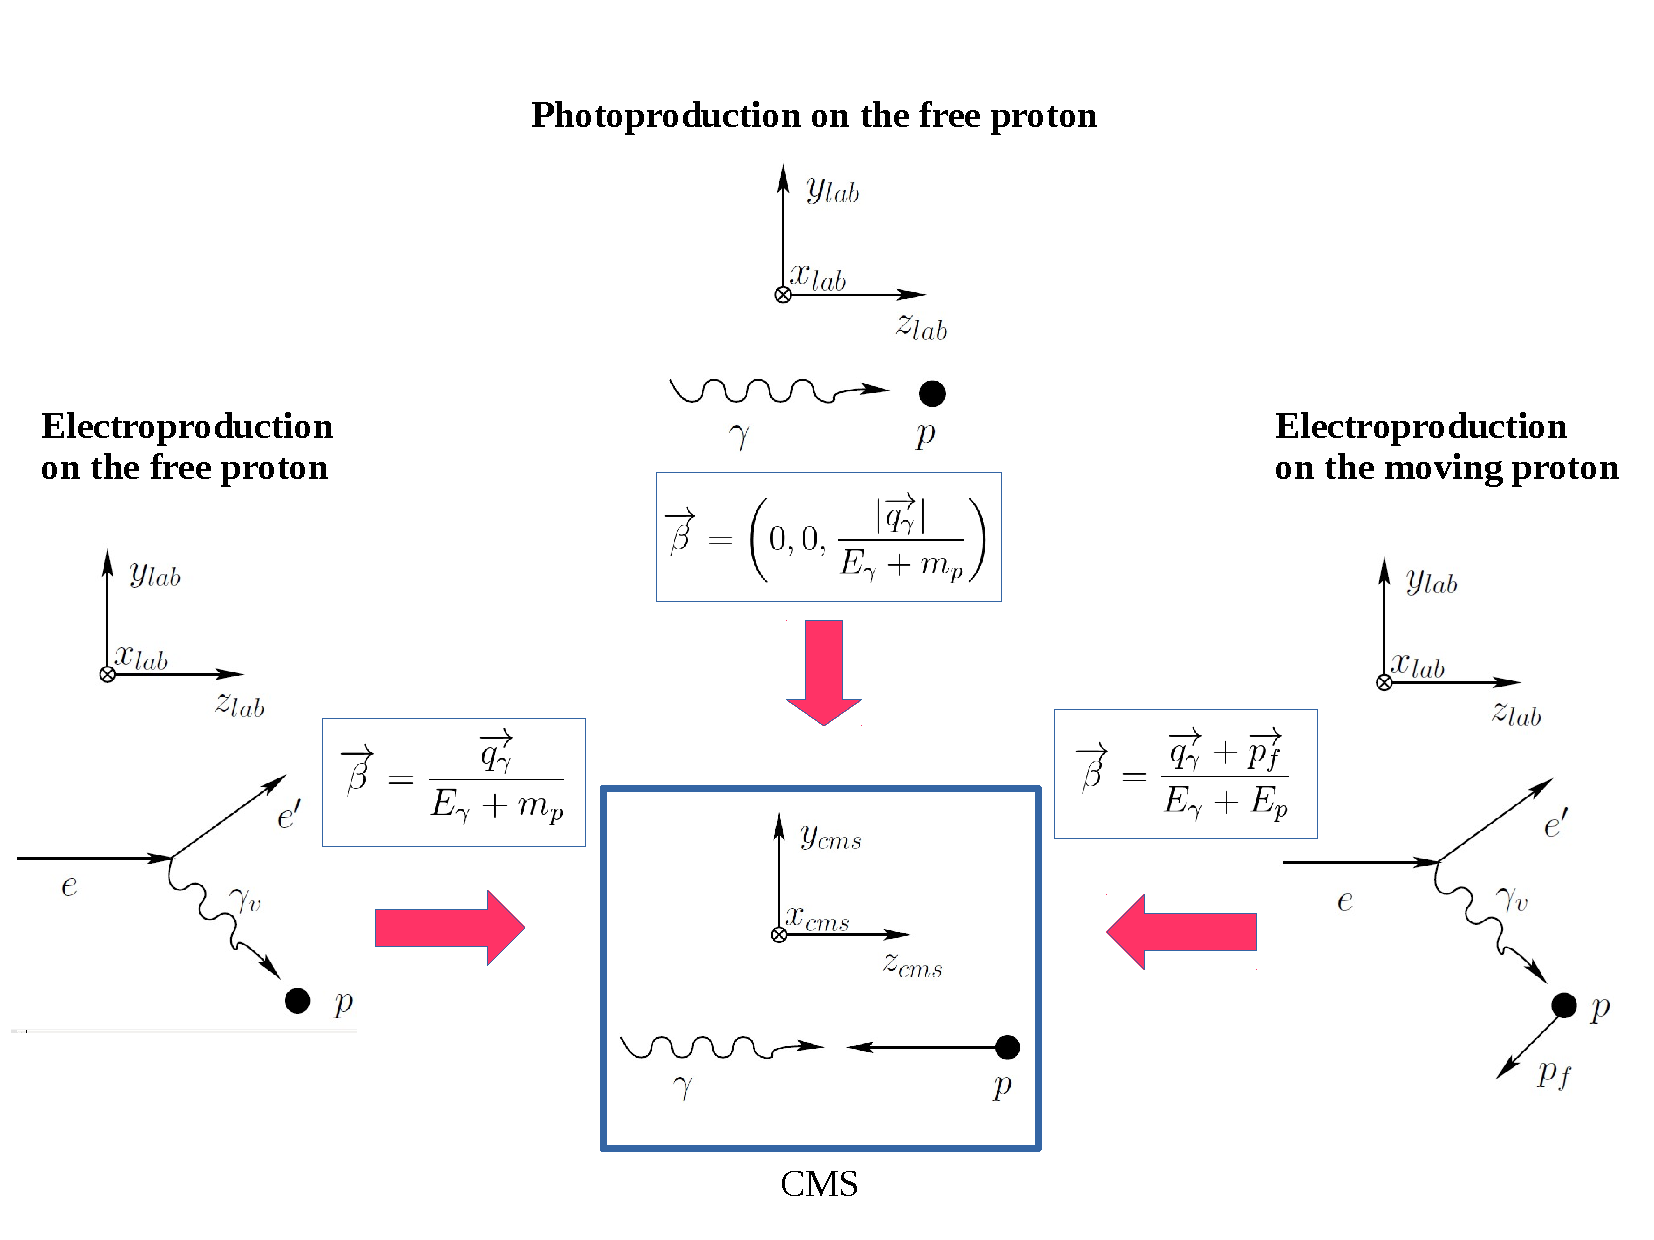
\includegraphics[width=13cm]{pictures/cross_section/lab_cms_trans2.pdf}}
\end{center}
\caption{\small  Illustration of three options for the experimental specification of the reaction initial state. Here $m_{p}$ is the proton mass, $\vec q_{\gamma}$ and $E_{\gamma}$ are the three-momentum and the energy of the interacting photon, respectively, while $p_{f}$ is the Fermi momentum of the target proton.}
\label{fig:lab_to_CMS}
\end{figure}


The correct procedure of the Lab to CMS transformation for an electroproduction experiment off a moving target (bottom right illustration in Fig.~\ref{fig:lab_to_CMS}) can be subdivided into two major steps.

\begin{enumerate}
\item First, one needs to perform the transition to the auxiliary system, where the target proton is at rest, while the incoming electron moves along the $z$-axis. This system is called ``quasi-Lab", since the initial conditions of the reaction in this frame imitate those existing in the Lab system in the case of the free proton experiment. The recipe of the Lab to quasi-Lab transformations is given in detail in Ref.~\cite{twopeg-d}.

\item Then, the quasi-Lab to CMS transformation should be performed by the standard method used for an electroproduction experiment off a proton at rest~\cite{Fed_an_note:2017} (bottom left illustration in Fig.~\ref{fig:lab_to_CMS}). Further details are given in App.~\ref{app_lab_cms_trans}.
\end{enumerate}


To perform the first step of this procedure (Lab to quasi-Lab transformation), one should be aware of the initial proton momentum for each reaction event~\cite{twopeg-d}. In this analysis, however, this information is available only in the fully exclusive topology, while the main $\pi^{-}$ missing topology lacks this information. This situation brings us to the impossibility to perform the correct Lab to CMS transformation for the majority of events. Therefore, in this analysis the procedure of Lab to CMS transformation for an electroproduction experiment off a proton at rest~\cite{Fed_an_note:2017} is used (bottom left illustration in Fig.~\ref{fig:lab_to_CMS}). The procedure is described in App.~\ref{app_lab_cms_trans}. This is done for both fully-exclusive and main $\pi^{-}$ missing topologies for consistency.

This approximation in the Lab to CMS transformation introduces a systematic inaccuracy to the extracted cross sections. A correction for this effect is included into the procedure of unfolding the effects of the target motion (see Sect.~\ref{Sect:fermi_corr}).




\clearpage


\section{Kinematic variables}
\label{Sect:kin_var}


When the four-momenta of all particles are defined and transformed to the CMS, one can calculate the kinematic variables that describe the reaction $ep(n) \rightarrow e'p'(n')\pi^{+}\pi^{-}$. For the description of the reaction initial state two variables are needed. In this study they are chosen in the following way: the invariant mass $W$, which is calculated according to Eq.~\eqref{W_fin_1}, and the photon virtuality $Q^{2}$, which is defined as
\begin{eqnarray}
Q^{2}= & -(P_{\gamma_{v}}^{\mu})^{2} = -(P_{e}^{\mu}-P_{e'}^{\mu})^{2}, \label{eq:q2} 
\end{eqnarray}
where $P_{\gamma_{v}}^{\mu}$ is the four-momentum of the virtual photon, while $P_{e}^{\mu}$ and $P_{e'}^{\mu}$ the four-momenta of the incoming and scattered electrons, respectively. 


The three-body final hadron state is unambiguously determined by five kinematic variables~\cite{Fed_an_note:2017}, and there are several options for their choice. The following generalized set of variables is used in this analysis\footnote[5]{More details on the organization of the reaction phase-space can be found in App.~\ref{app_ph_space}.}:\vspace{-0.5em}

\begin{itemize}
\item invariant mass of the first pair of the hadrons $M_{h_{1}h_{2}}$,\vspace{-0.4em}
\item invariant mass of the second pair of the hadrons $M_{h_{2}h_{3}}$,\vspace{-0.4em}
\item the first particle solid angle $\Omega_{h_{1}} = (\theta_{h_{1}}, \varphi_{h_{1}})$, and\vspace{-0.4em}
\item the angle $\alpha_{h_{1}}$ between the two planes (i) defined by the three-momenta of the virtual photon (or initial proton) and the first final hadron and (ii) defined by the three-momenta of all final hadrons\footnote[6]{Note that the three-momenta of the $\pi^{+}$, $\pi^{-}$, $p'$ are in the same plane, since in the CMS their total three-momentum has to be equal to zero.}.\vspace{-0.5em}
\end{itemize}

The cross sections in this analysis are obtained in three sets of variables depending on various assignments for the first, second, and third final hadrons:\vspace{-0.5em}
\begin{itemize}
\item[1.] [$p'$, $\pi^{+}$, $\pi^{-}$]
$M_{p'\pi^{+}}$, $M_{\pi^{+}\pi^{-}}$, $\theta_{p'}$~,~$\varphi_{p'}$~,~$\alpha_{p'}$~~(or $\alpha_{[pp'][\pi^{+}\pi^{-}]}$),\vspace{-0.25em}

\item[2.] [$\pi^{-}$, $\pi^{+}$, $p'$]
$M_{\pi^{-}\pi^{+}}$, $M_{\pi^{+}p'}$, $\theta_{\pi^{-}}$, $\varphi_{\pi^{-}}$, $\alpha_{\pi^{-}}$ (or $\alpha_{[p\pi^{-}][p'\pi^{+}]}$),\vspace{-0.25em}


\item[3.]  [$\pi^{+}$, $\pi^{-}$, $p'$]
$M_{\pi^{+}\pi^{-}}$, $M_{\pi^{-}p'}$, $\theta_{\pi^{+}}$, $\varphi_{\pi^{+}}$, $\alpha_{\pi^{+}}$ (or $\alpha_{[p\pi^{+}][p'\pi^{-}]}$).\vspace{-0.5em}
\end{itemize}


Lets explain in more detail the calculation of the kinematic variables for the case of the set number two. The invariant masses $M_{\pi^{+}\pi^{-}}$ and $M_{\pi^{+}p'}$ are calculated from the four-momenta of the final particles $P_{\pi^{-}}^{\mu}$, $P_{\pi^{+}}^{\mu}$, $P_{p'}^{\mu}$ in the following way:
\begin{equation}
\begin{aligned}
M_{\pi^{+}\pi^{-}} = \sqrt{(P_{\pi^{+}}^{\mu} + P_{\pi^{-}}^{\mu})^{2}} & \text{~~~~and}\\ \label{invmasses}
M_{\pi^{+}p'} = \sqrt{(P_{\pi^{+}}^{\mu} + P_{p'}^{\mu})^{2}}. & \\ 
\end{aligned}  
\end{equation}  


The polar ($\theta_{\pi^{-}}$) and azimuthal ($\varphi_{\pi^{-}}$) angles of the $\pi^{-}$ in the CMS are shown in Fig.~\ref{fig:cr_sec_thetaphi}. In this figure the $z$-axis is directed along the virtual photon (with the unit vector $\vec n_{z}$), while the $x$-axis is located in the electron scattering plane and follows the direction of the scattered electron (see App.~\ref{app_lab_cms_trans} for details). The plane $A$ in Fig.~\ref{fig:cr_sec_thetaphi} is defined by the three-momenta of the $\pi^{-}$ and initial proton.  
	
The angle $\theta_{\pi^{-}}$ varies in the range $[0,\pi]$ and is calculated as:%\vspace{-0.25em}
\begin{equation}
\theta_{\pi^{-}} = \arccos\left( \frac{(\vec P_{\pi^{-}} \cdot \vec P_{\gamma})}
{|\vec P_{\pi^{-}}| |\vec P_{\gamma}|} \right),
\label{angletheta}
\end{equation} 
where $\vec P_{\gamma}$ is the three-momentum of the virtual photon and $\vec P_{\pi^{-}}$ is the three-momentum of the  $\pi^{-}$ (both are situated in the plane $A$).

The angle $\varphi_{\pi^{-}}$ varies in the range $[0,~2\pi]$ and is determined as:
\begin{equation}
\begin{aligned}
\varphi_{\pi^{-}} &= \arctan\left( \frac{P_{y}}{P_{x}} \right), &\text{~~if~~} P_{x} > 0 \text{~~and~~}  P_{y} > 0, \\
\varphi_{\pi^{-}} &= \arctan\left( \frac{P_{y}}{P_{x}} \right) + 2\pi, &\text{~~if~~}P_{x} > 0 \text{~~and~~}  P_{y} < 0, \\
\varphi_{\pi^{-}} &= \arctan\left( \frac{P_{y}}{P_{x}} \right) + \pi, &\text{~~if~~}P_{x} < 0 \text{~~and~~}  P_{y} < 0, \\
\varphi_{\pi^{-}} &= \arctan\left( \frac{P_{y}}{P_{x}} \right) + \pi, &\text{~~if~~}P_{x} < 0 \text{~~and~~}  P_{y} > 0,  \\
\varphi_{\pi^{-}} &= \frac{\pi}{2}, &\text{~~if~~}P_{x} = 0 \text{~~and~~}  P_{y} > 0,  \\
\varphi_{\pi^{-}} &= \frac{3\pi}{2}, &\text{~~if~~}P_{x} = 0\text{~~and~~}  P_{y} < 0, 
\end{aligned}
\end{equation}
where $P_{i}$ is the $i$-component of the $\pi^{-}$ three-momentum in the CMS ($i = x,y,z$).

The calculation of the angle $\alpha_{\pi^{-}}$, which is shown in Fig.~\ref{fig:cr_sec_kinematic2}, is more complicated. This is the angle between the two planes A and B, which varies in a range $[0,~2\pi]$. The plane A is defined by the three-momentum of the initial proton and the three-momentum of the $\pi^{-}$. The plane B is defined by the three-momenta of all final hadrons. For the calculation of the $\alpha_{\pi^{-}}$, one determines first three auxiliary vectors $\vec \gamma$, $\vec \beta$, and $\vec \delta$, which are also shown in Fig.~\ref{fig:cr_sec_kinematic2}.

%\clearpage
\begin{figure}[htp]
\begin{center}
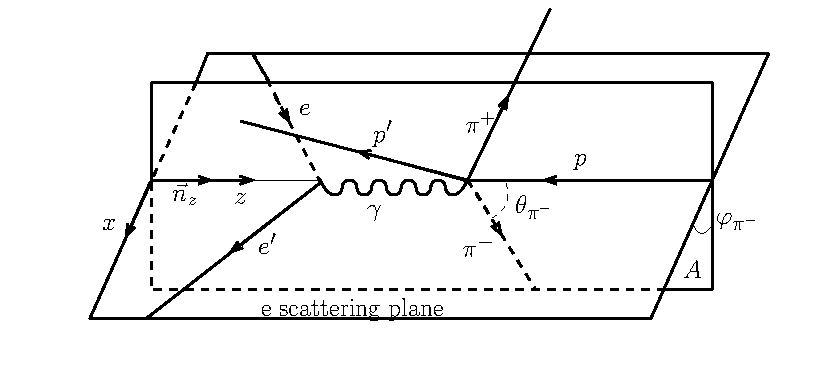
\includegraphics[width=14cm]{pictures/cross_section/thetaphi_new.pdf}
\caption{\small Polar ($\theta_{\pi^{-}}$) and azimuthal ($\varphi_{\pi^{-}}$) angles of the $\pi^{-}$ in the CMS. The $z$-axis is directed along the virtual photon (with the unit vector $\vec n_{z}$), while the $x$-axis is located in the electron scattering plane and follows the direction of the scattered electron. The plane $A$ is defined by the three-momenta of the $\pi^{-}$ and initial proton. } \label{fig:cr_sec_thetaphi}
\end{center}
\end{figure}
\begin{figure}[htp]
\begin{center}
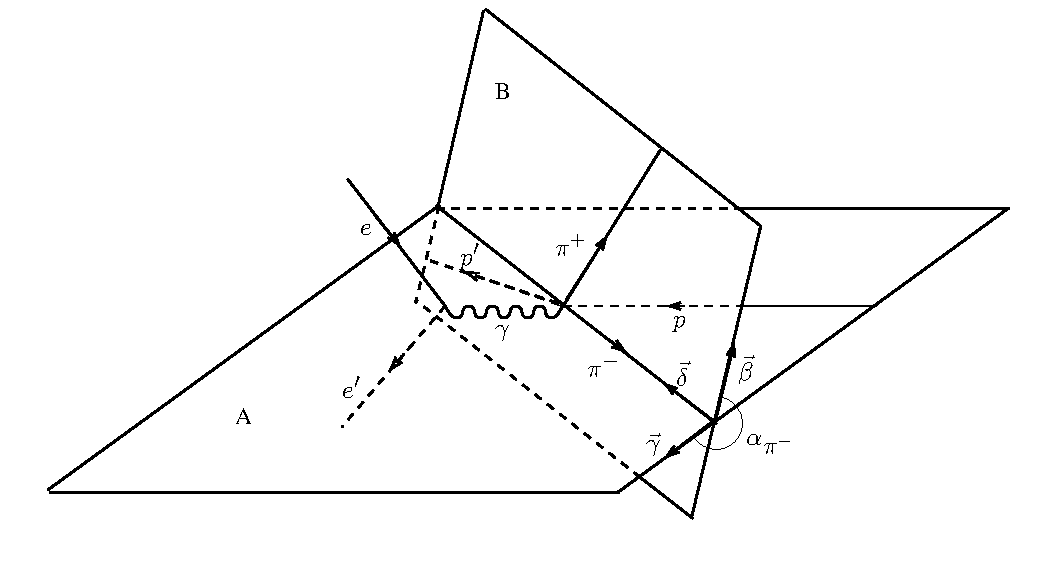
\includegraphics[width=14cm]{pictures/cross_section/alpha1.pdf}
\caption{\small Definition of the angle $\alpha_{\pi^{-}}$ between the two planes: the plane A is defined by  the three-momenta of the $\pi^{-}$ and initial proton, while the plane B is defined by the three-momenta of all final hadrons. The definitions of  auxiliary vectors $\vec \beta$, $\vec \gamma$, and $\vec \delta$ are given in the text.} \label{fig:cr_sec_kinematic2}
\end{center}
\end{figure}



The auxiliary unit vector $\vec \gamma$ is situated in the plane A. This vector is perpendicular to the three-momentum of the $\pi^{-}$ and directed toward the vector $[-\vec n_{z}]$, where $\vec n_{z}$ is the unit vector directed along the $z$-axis. The vector $\vec \gamma$ can be expressed as

\begin{gather*}
\vec \gamma = a_{\alpha}\cdot[-\vec n_{z}]~+~b_{\alpha}\cdot\vec n_{\pi^{-}}  \nonumber \\[10pt]
\text{with~~~}a_{\alpha}  =\sqrt{\frac{1}{1 - (\vec n_{\pi^{-}} \cdot [-\vec n_{z}] )^{2}}}  \text{~~~and~~~} \label{alphavec}
b_{\alpha}  = -  a_{\alpha}\cdot \left (\vec n_{\pi^{-}} \cdot [-\vec n_{z}] \right) \textrm{ ,} \nonumber
\end{gather*}
where $\vec n_{\pi^{-}}$ is the unit vector directed along the three-momentum of the $\pi^{-}$. 



The auxiliary unit vector $\vec \beta$ is situated in the plane B. This vector is perpendicular to the three-momentum of the $\pi^{-}$ and directed toward the three-momentum of the $\pi^{+}$. The vector $\vec \beta$ can be expressed as
\begin{gather*}
\vec \beta = a_{\beta}\cdot\vec n_{\pi^{+}}~+~b_{\beta}\cdot\vec n_{\pi^{-}}  \nonumber \\[10pt]  
\text{with~~~}a_{\beta} = \sqrt{\frac{1}{1 - (\vec n_{\pi^{+}} \cdot \vec n_{\pi^{-}})^{2}}} \text{~~~and~~~} \label{betavec}
b_{\beta} = -  a_{\beta}\cdot(\vec n_{\pi^{+}} \cdot \vec n_{\pi^{-}}) \textrm{ ,} \nonumber
\end{gather*} 
where $\vec n_{\pi^{+}}$ is the unit vector directed along the three-momentum of the $\pi^{+}$. 

Taking the scalar products $(\vec \gamma \cdot \vec  \gamma)$, $(\vec \beta \cdot \vec  \beta)$, $(\vec \gamma \cdot \vec n_{\pi^{-}})$, and $(\vec \beta \cdot \vec n_{\pi^{-}})$, it is straightforward to verify that $\vec \gamma$ and $\vec  \beta$ are the unit vectors perpendicular to the three-momentum of the $\pi^{-}$.

The auxiliary unit vector $\vec \delta$ is the vector product of the auxiliary vectors $\vec \gamma$ and $\vec \beta$, i.e. 
\begin{equation}
\vec \delta = [ \vec \gamma \times \vec \beta ].
\end{equation}

Then the angle $\alpha_{\pi^{-}}$ is determined as:
\begin{equation}
\begin{aligned}
\alpha_{\pi^{-}} &= \arccos(\vec \gamma \cdot \vec \beta),&\text{~~if~~~} \vec \delta~\uparrow\uparrow~\vec n_{\pi^{-}},\\
\alpha_{\pi^{-}} &= 2\pi - \arccos(\vec \gamma \cdot \vec \beta),&\text{~~if~~~} \vec \delta~\uparrow\downarrow~\vec n_{\pi^{-}}.    \label{eq:cr_sec_anglealpha}
\end{aligned}
\end{equation}

The kinematic variables for the first and third sets are calculated in a similar way. The angles $\alpha_{p'}$ and $\alpha_{\pi^{+}}$ are shown for the convenience in Figs.~\ref{fig:cr_sec_kinematic1} and ~\ref{fig:cr_sec_kinematic3}. Further information on the kinematic of reactions with multi-particle final states can be found in Ref.~\cite{Byckling:1971vca}.


%\clearpage
\begin{figure}[htp]
\begin{center}
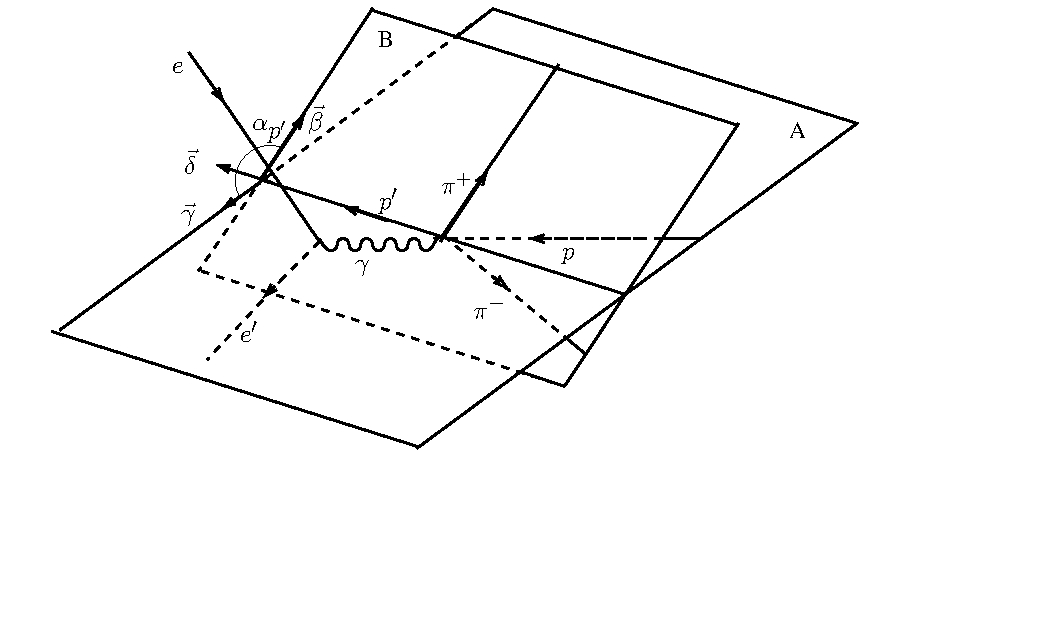
\includegraphics[width=12cm]{pictures/cross_section/alpha2.pdf}
\caption{\small Definition of the angle $\alpha_{p'}$ between the two planes:  the plane A is defined by the three-momenta of initial and scattered protons, while the plane B is defined by the three-momenta of all final hadrons.} \label{fig:cr_sec_kinematic1}
\end{center}
\end{figure}
\begin{figure}[htp]
\begin{center}
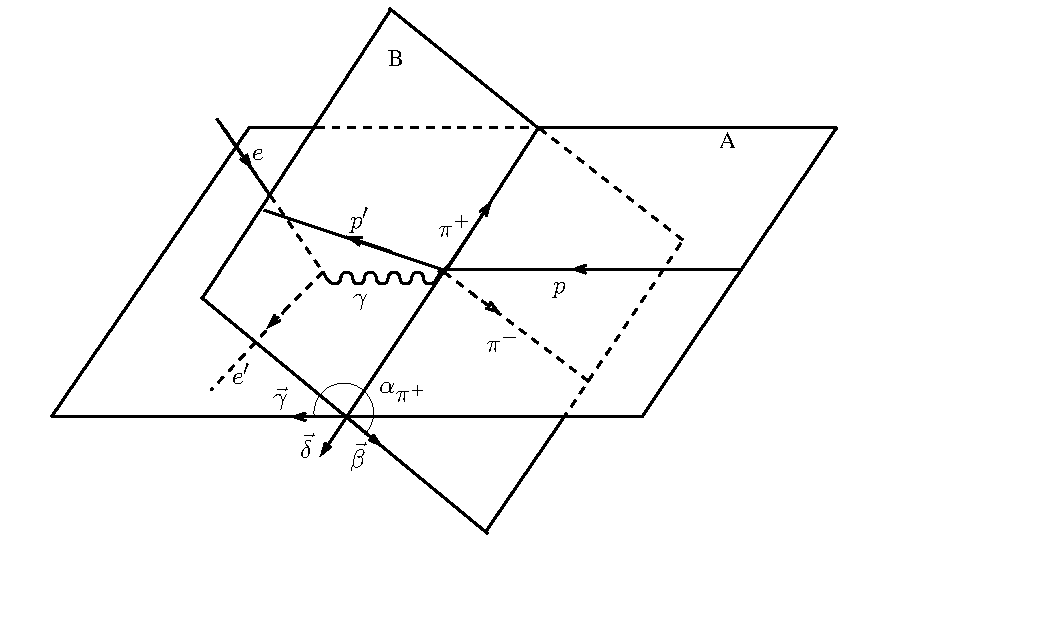
\includegraphics[width=12cm]{pictures/cross_section/alpha3.pdf}
\caption{\small Definition of the angle $\alpha_{\pi^{+}}$ between the two planes: the plane A is defined by the three-momenta of the $\pi^{+}$ and initial proton, while the plane B is defined by the three-momenta of all final hadrons.} \label{fig:cr_sec_kinematic3}
\end{center}
\end{figure}
\clearpage



\section{Binning and kinematic coverage}
\label{Sect:binning}

The available kinematic coverage in the initial state variables is shown by the $Q^2$ versus $W$ distribution\footnote[7]{Note that $W$ here is $W_{sm}$, and therefore, the distribution boundaries are not subject to the blurring. See Sect.~\ref{Sect:smearing_blurring} for details.} in Fig.~\ref{fig:q2_vs_w}. This distribution is filled with the double-pion events survived after the event selection described above. The blue boundary limits the analyzed kinematic area, where the double-pion cross sections are extracted. The black grid demonstrates the chosen binning in the initial state variables (25~MeV in $W$ and 0.05~GeV$^{2}$ in $Q^{2}$).



\begin{figure}[htp]
\begin{center}
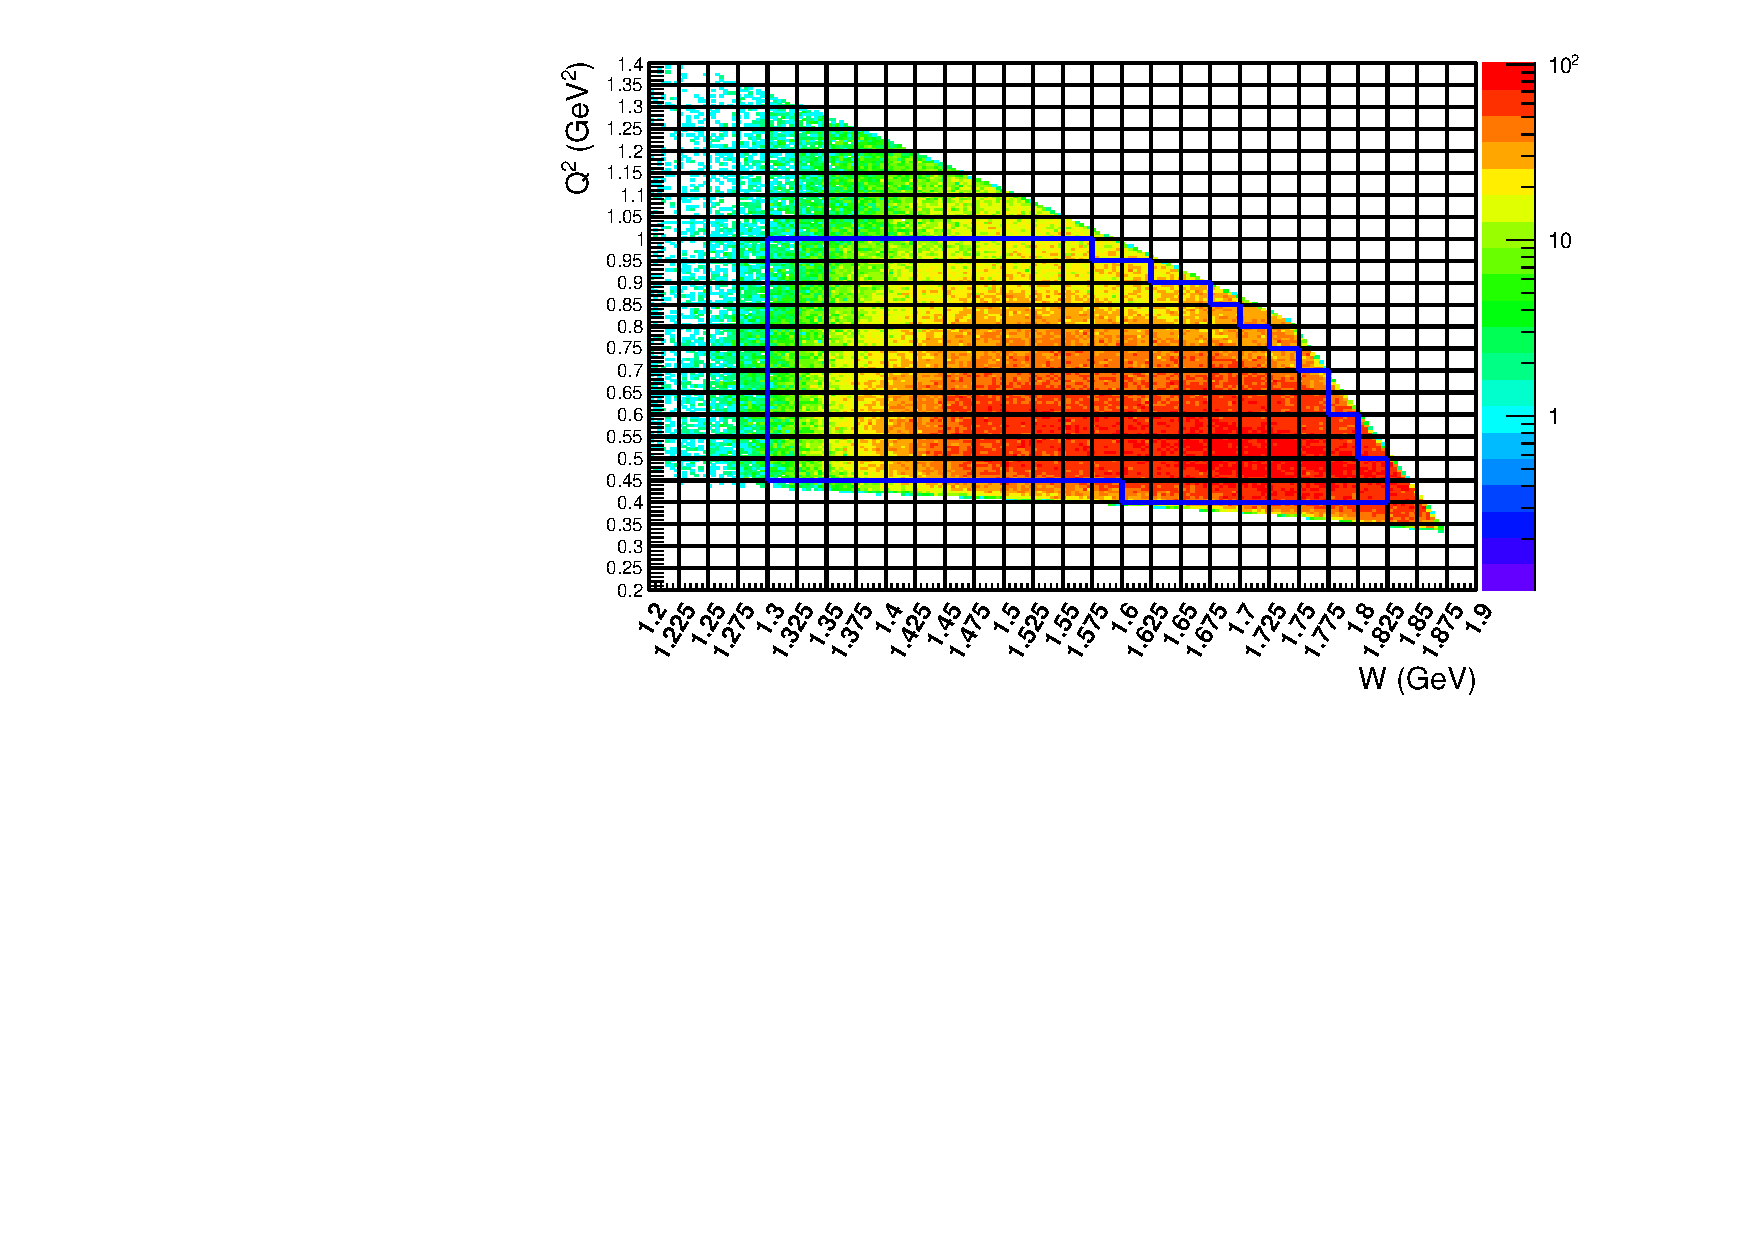
\includegraphics[width=0.95\textwidth]{pictures/cross_section/q2vsw_new.pdf}
\caption{\small $Q^2$ versus $W$ distribution populated with the selected double-pion events. The cross section is calculated in 2D cells within the blue boundaries.} \label{fig:q2_vs_w}
\end{center}
\end{figure}

The kinematic coverage in the final state variables has the following reaction related features. The angular variables $\theta_{h_{1}}$, $\varphi_{h_{1}}$, and $\alpha_{h_{1}}$ vary in the fixed ranges of $[0,~\pi]$, $[0,~2\pi]$, and $[0,~2\pi]$, respectively. Meanwhile, the ranges of the invariant masses $M_{h_{1}h_{2}}$ and $M_{h_{2}h_{3}}$ are $W$ dependent and broaden as $W$ grows. More details on the specificity of the double-pion production phase-space are given in App.~\ref{app_ph_space}. 

The binning in the final hadron variables used in this study is listed in Tab.~\ref{tab:summary_bins}. In each $W$ and $Q^{2}$ bin the range of each final hadron variable is divided into bins of equal size. However, the number of bins differs in various $W$ subranges, in order to take into account (i) the statistics drop near the reaction threshold, which is at $\approx$~1.22~GeV and (ii) the aforementioned broadening of the reaction phase-space with increasing $W$. The chosen amount of bins in each considered $W$ subrange reflects the intention to maintain reasonable statistical uncertainties of the single-differential cross sections for all $W$ and $Q^2$ bins. 



For the binning in the polar angle note the following. The cross section, although being differential in $[-\cos\theta]$, is binned in $\theta$. These $\Delta \theta$ bins are of equal size in the corresponding $W$ subrange. See also Sect.~\ref{Sect:cr_sect_formula} on this matter.



\vspace{0.5em}
\begin{table}[htb]
\centering 
  \caption{Number of bins for hadronic variables.} \label{tab:summary_bins}
  \begin{tabular}{lm{4cm}cccc}
    \toprule
    & & \multicolumn{4}{c}{W subrange (GeV)} \\
    \multicolumn{2}{c}{\centering Hadronic variable }  & [1.3,~1.35] & [1.35,~1.4] & [1.4,~1.475] & [1.475,~1.825] \\
    \cmidrule(l{5pt}r{15pt}){1-2} \cmidrule(l{5pt}r{5pt}){3-6}
    $M_{h_{1}h_{2}}$   & Invariant mass       &   8  & 10 & 12 & 12  \\
    $M_{h_{2}h_{3}}$   & Invariant mass       &   8  & 10 & 12 & 12  \\
    $\theta_{h_{1}}$   & Polar angle          &   6  & 8  & 10 & 10  \\
    $\varphi_{h_{1}}$  & Azimuthal angle      &   5  & 5  & 5  & 6   \\
    $\alpha_{h_{1}}$   & Angle between planes &   5  & 6  & 8  & 8   \\
    \cmidrule(l{5pt}r{15pt}){1-2} \cmidrule(l{5pt}r{5pt}){3-6}
              & Total number of bins \newline in hadronic variables &   9600  & 24000  & 57600  & 69120   \\
    \bottomrule
  \end{tabular}
\end{table}
\vspace{0.5em}

The total numbers of multi-dimensional bins for the corresponding $W$ ranges are listed in the last row of Tab.~\ref{tab:summary_bins} and require some clarification. In fact the invariant masses border of the double-pion production phase-space is $W$-dependent and determined by the Byckling function (see App.~\ref{app_ph_space}). Therefore, the bins located outside this border contain no double-pion events and hence do not contribute to the cross section. For a given $W$ value, the border is distinct, however for a $W$ bin, which corresponds to a range of $W$ values, it is somewhat diffused. If events are binned in $W_{true}$ (like in a free proton experiment) and the bin is small, e.g. 25 MeV, this diffusion is marginal. Then the quantity of bins involved in the cross section calculation (including both non-empty and empty cells) varies from 90\% to 70\% of the total numbers given in the last row of Tab.~\ref{tab:summary_bins} as $W$ increases from the threshold. However, if events are binned in $W_{sm}$ (like in this analysis), each $W_{sm}$ value in a bin corresponds to a sequence of $W_{true}$ spread over 50-100 MeV. In this case a very pronounced boundary diffusion takes place, increasing the quantity of bins filled with events, i.e. the fraction of bins involved in the cross section calculation turn out to vary from 100\% to 80\% as $W$ increases\footnote[8]{This estimation is based on the Monte Carlo simulation performed with TWOPEG~\cite{twopeg} and TWOPEG-D~\cite{twopeg-d} for the reactions off the proton at rest and off the moving proton, respectively.}.



The specific organization of the double-pion production phase-space in the invariant masses $(M_{h_{1}h_{2}}, M_{h_{2}h_{3}})$ causes the need to pay special attention to the binning in these variables. Equation~\eqref{eq:inv_mass_boundary} gives the expressions for the lower and upper boundaries of the $M_{h_{1}h_{2}}$ distribution and demonstrates that the upper boundary depends on the value of $W$, while the lower does not (see also App.~\ref{app_ph_space} on this matter).
\begin{equation}
\begin{aligned}
M_{lower} &= m_{h_1} + m_{h_2} \\
M_{upper} (W) &= W - m_{h_3}. \label{eq:inv_mass_boundary}
\end{aligned}  
\end{equation}

Here $m_{h_1}$, $m_{h_2}$, and $m_{h_3}$ are the masses of the final hadrons. 


Since the cross section is calculated in a bin $W_{left} < W < W_{right}$, the boundary of $M_{upper}$ is not distinct. For the purpose of binning in mass, the value of $M_{upper}$ is calculated using $W_{center}$, at the center of the $W$ bin. As a result, some events with $W > W_{center}$ turned out to be located beyond $M_{upper}$. Hence it was decided to use a specific arrangement of mass bins with the bin width $\Delta M$ determined by
\begin{equation}
\begin{aligned}
\Delta M = \frac{M_{upper}-M_{lower}}{N_{bins}-1}, \label{eq:bin_width}
\end{aligned}  
\end{equation} 
where $N_{bins}$ is the number of bins specified in the first row of Tab.~\ref{tab:summary_bins}. The left boundary of the first bin is set to $M_{lower}$.

The chosen arrangement of bins forces the last bin to be situated completely out of the boundaries\footnote[9]{Note that for each $W$ bin and for each invariant mass, $\Delta M$ given by Eq.~\eqref{eq:bin_width} is greater than 12.5~MeV, which is the half of the $W$ bin width.} given by Eq.~\eqref{eq:inv_mass_boundary} using $W_{center}$. Therefore, the cross section in this extra bin finally is not reported. However, this bin is kept in the analysis since its content (though being very small) contributes to all cross sections that are obtained by integrating over the corresponding invariant mass distribution. 


Note that the cross section in the next to last bin in invariant mass needs a special correction. This correction is described in Sect.~\ref{Sect:bin_cor}.



%===============================================

\section{Cross section formulae}
\label{Sect:cr_sect_formula}

\subsection{Electron scattering cross section}

The experimental electron scattering cross section $\sigma_{e}$ for the reaction $ep(n) \rightarrow e'p'(n') \pi^{+} \pi^{-}$ is seven-fold differential and calculated as\footnote[10]{To deal with the multi-differential cross section, THnSparse multi-dimensional root histograms are used.}
\begin{equation}
\frac{\textrm{d}^{7}\sigma_{e}}{\textrm{d}W\textrm{d}Q^{2}\textrm{d}^{5}\tau} = \frac{1}{ R \! \cdot \! \mathcal{F}}  \cdot 
\frac{\left( \frac{N_{full}}{Q_{full}}-\frac{N_{empty}}{Q_{empty}} \right)}{
\Delta W \! \cdot \! \Delta Q^{2} \! \cdot \! \Delta^{5} \tau \! \cdot \! \left[ \frac{l \cdot \rho \cdot N_{A}}{q_{e}\cdot \mu_{d}} \right]\! \cdot \!\mathcal{E}} \textrm{ , where}
\label{expcrossect}
\end{equation}
%where
%\vspace{-2.4em}
\begin{itemize}
\item $\textrm{d}^{5}\tau = \textrm{d}M_{h_{1}h_{2}} \textrm{d}M_{h_{2}h_{3}} \textrm{d}\Omega_{h_1} \textrm{d}\alpha_{h_1}$ is the differential of the five independent variables of the $\pi^{+}\pi^{-}p$ final state, which are described in Sect.~\ref{Sect:kin_var};\vspace{-0.25em}
\item $N_{full}$ and $N_{empty}$ are the numbers of selected double-pion events inside the seven-dimensional bin for runs with deuterium and empty target, respectively;\vspace{-0.25em} 
\item the quantity in the square brackets in the denominator corresponds to the luminosity of the experiment $\mathcal{L}$ in the units cm$^{-2}\cdot$C$^{-1}$ and its components are\vspace{-0.25em}
\begin{itemize}
\item [ ]  $l$ = 2 cm the length of the target,\vspace{-0.4em}
\item [ ]  $\rho$ = 0.169 g$\cdot$cm$^{-3}$ the density of liquid deuterium,\vspace{-0.4em}
\item [ ]  $N_{A}$ = 6.022$\cdot 10^{-19}$ mol$^{-1}$ Avogadro's number,\vspace{-0.4em}
\item [ ]  $q_{e}$ = 1.602$\cdot 10^{-19}$ C the elementary charge, and \vspace{-0.4em}
\item [ ]  $\mu_{d}$ = 2.014 g$\cdot$mol$^{-1}$ the molar mass of deuterium,\vspace{-0.25em}
\end{itemize}
which results in the luminosity value of $\mathcal{L}$ = 0.63$\cdot$10$^{42}$ cm$^{-2}\cdot$C$^{-1}$ = 0.63$\cdot$10$^{12}$ $\mu$b$^{-1}\cdot$C$^{-1}$;\vspace{-0.25em}


\item $Q_{full}$ = 3734.69 $\mu C$ and $Q_{empty}$ = 464.797 $\mu C$ are the values of the charge accumulated in the Faraday Cup for deuterium and empty target runs, respectively\footnote[11]{They are calculated by summing up the charges of all analyzed \textit{blocks} (see Sect.~\ref{Sect:qcheck} for details).}, which results in the corresponding values of the integrated luminosity $L=\mathcal{L}\cdot Q$ of 2.35$\cdot 10^{9}$ $\mu \text{b}^{-1}$ and 0.29$\cdot 10^{9}$ $\mu \text{b}^{-1}$; \vspace{-0.25em}

\item $\mathcal{E} = \mathcal{E}(\Delta W, \Delta Q^{2}, \Delta^{5}\tau)$ is the detector efficiency (which includes the detector acceptance) for each seven-dimensional bin as determined by the Monte Carlo simulation (see Sect.~\ref{Sect:eff_eval}); \vspace{-0.25em}

\item $R = R(\Delta W, \Delta Q^{2})$ is the radiative correction factor described in Sec.~\ref{Sect:rad_corr}; \vspace{-0.25em}

\item $\mathcal{F} = \mathcal{F}(\Delta W, \Delta Q^{2}, \Delta^{5}\tau)$ is the correction factor that aims at unfolding the effects of the target motion (see Sect.~\ref{Sect:fermi_corr}).

\end{itemize}

The electron scattering cross section $\sigma_{e}$ in the left hand side of Eq.~\eqref{expcrossect} is assumed to be obtained in the center of the finite seven-dimensional kinematic bin $\Delta W \Delta Q^{2} \Delta^{5} \tau$. 



\subsection{Virtual photoproduction cross section}

The goal of the analysis is to extract the virtual photoproduction cross section $\sigma_{v}$ of the reaction $\gamma_{v}p(n) \rightarrow p'(n') \pi^{+} \pi^{-}$. This virtual photoproduction cross section $\sigma_{v}$ is five-fold differential and in the single-photon exchange approximation connected with the seven-fold differential electron scattering cross section\footnote[12]{Note that after the corrections introduced in Eq.~\eqref{expcrossect} by the factors $R$ and $\mathcal{F}$, the cross section $\sigma_{e}$ is the true electron scattering cross section attributed to the central values of the corresponding $\Delta W \Delta Q^{2} \Delta^{5} \tau$ bin and the distinct value of the beam energy $E_{beam} = 2.039$~GeV.} $\sigma_{e}$ via 
\begin{equation}
\begin{aligned}
\frac{\textrm{d}^{5}\sigma_{v}}{\textrm{d}^{5}\tau} &= \frac{1}{\Gamma_{v}}\frac{\textrm{d}^{7}\sigma_{e}}{\textrm{d}W\textrm{d}Q^{2}\textrm{d}^{5}\tau}  \textrm{ ,}
\end{aligned} 
\label{fulldiff}
\end{equation}
where $\Gamma_{v}$ is the virtual photon flux given by
\begin{equation}
\Gamma_{v} (W, Q^2) =
\frac{\alpha}{4\pi}\frac{1}{E_{beam}^{2}m_{p}^{2}}\frac{W(W^{2}-m_{p}^{2})}
{(1-\varepsilon_{T})Q^{2}} \textrm{ .}
\label{flux}
\end{equation}

Here $\alpha$ is the fine structure constant $\left(1/137\right)$, $m_{p}$ the proton mass, $E_{beam}$ = 2.039 GeV the laboratory energy of the incoming electron beam, and $\varepsilon_{T}$ the virtual photon transverse polarization given by \vspace{-1em}
\begin{equation}
\varepsilon_{T} = \left( 1 + 2\left( 1 +
\frac{\nu^{2}}{Q^{2}} \right)
\tan^{2}\left(\frac{\theta_{e'}}{2}\right) \right)^{-1} \textrm{ ,}
\label{polarization}
\end{equation}
where $\nu = E_{beam} - E_{e'}$ is the virtual photon energy, while $E_{e'}$ and $\theta_{e'}$ are the energy and the polar angle of the scattered electron in the lab frame, respectively. 
%$W$, $Q^{2}$ and $\theta_{e'}$ are taken in the center of the bin.

The value of the virtual photon flux given by Eq.~\eqref{flux} is calculated for the central point of the $\Delta W \Delta Q^{2}$ bin. %Note that the $\Gamma_{v}$ is calculated using the smeared value of $W$. A correction for this approximation is included into the procedure of unfolding the effects of the target motion (see Sect.~\ref{Sect:fermi_corr}). Therefore, $\sigma_{v}$ in the left hand side of the Eq.~\eqref{fulldiff} is attributed to the non-smeared value of $W$. 

The limited statistics of the experiment does not allow for estimates of the five-fold differential cross section $\sigma_{v}$ with a reasonable accuracy. Therefore, the cross section $\sigma_{v}$ is first obtained on the multi-dimensional grid and then is integrated over at least four hadron variables. Hence, only the sets of the single-differential and fully-integrated cross sections are obtained.


%being obtained on the multi-dimensional grid, the cross section $\sigma_{v}$ is then 

For each $W$ and $Q^{2}$ bin, the following cross sections are extracted for each variable set.
\begin{equation}
\begin{aligned}
\frac{\textrm{d}\sigma_{v}}{\textrm{d}M_{h_{1}h_{2}}} & =\int\frac{\textrm{d}^{5}\sigma_{v}}{\textrm{d}^{5}\tau}\textrm{d}M_{h_{2}h_{3}}\textrm{d}\Omega_{h_{1}}\textrm{d}\alpha_{h_{1}}, \\
\frac{\textrm{d}\sigma_{v}}{\textrm{d}M_{h_{2}h_{3}}} & =\int\frac{\textrm{d}^{5}\sigma_{v}}{\textrm{d}^{5}\tau}\textrm{d}M_{h_{1}h_{2}}\textrm{d}\Omega_{h_{1}}\textrm{d}\alpha_{h_{1}}, \\
\frac{\textrm{d}\sigma_{v}}{\textrm{d}[-\cos\theta_{h_{1}}]} & =\int\frac{\textrm{d}^{5}\sigma_{v}}{\textrm{d}^{5}\tau}\textrm{d}M_{h_{1}h_{2}}\textrm{d}M_{h_{2}h_{3}}\textrm{d}\varphi_{h_{1}}d\alpha_{h_{1}}, \\
\frac{\textrm{d}\sigma_{v}}{\textrm{d}\alpha_{h_{1}}} & =\int\frac{\textrm{d}^{5}\sigma_{v}}{\textrm{d}^{5}\tau}\textrm{d}M_{h_{1}h_{2}}\textrm{d}M_{h_{2}h_{3}}\textrm{d}\Omega_{h_{1}},~~\text{and}\\
\sigma_{v}^{int} (W, Q^{2}) &= \int \frac{d^{5}\sigma_{v}}{\textrm{d}^{5}\tau}\textrm{d}M_{h_{1}h_{2}}\textrm{d}M_{h_{2}h_{3}}\textrm{d}\Omega_{h_{1}}\textrm{d}\alpha_{h_{1}}.
\end{aligned}
\label{inegr5diff}
\end{equation}

%!!! Since the cross sections are obtained on the five-dimensional kinematic grid, the integrals in Eqs.~\eqref{inegr5diff} are calculated numerically on that grid. 

As a final result for each $W$ and $Q^{2}$ bin, the integral cross section $\sigma_{v}^{int}$, averaged over the three variable sets, is reported together with the nine single-differential cross sections given in \eqref{eq:reported_sec}, where each column is taken from the corresponding variable set.
\begin{equation}
\begin{aligned}
&~~~~~~\frac{\textrm{\textrm{d}}\sigma_{v}}{\textrm{d}M_{p'\pi^{+}}}&&~~~~~~\frac{\textrm{d}\sigma_{v}}{\textrm{d}M_{\pi^{-}\pi^{+}}}&&~~~~~~\frac{\textrm{d}\sigma_{v}}{\textrm{d}M_{\pi^{-}p'}}\\[8pt] 
&~~\frac{\textrm{d}\sigma_{v}}{\textrm{d}[-\cos\theta_{p'}]}&&~~\frac{\textrm{d}\sigma_{v}}{\textrm{d}[-\cos\theta_{\pi^{-}}]}&&~~\frac{\textrm{d}\sigma_{v}}{\textrm{d}[-\cos\theta_{\pi^{+}}]}\\[8pt] 
&~~~~~~~\frac{\textrm{d}\sigma_{v}}{\textrm{d}\alpha_{p'}}&&~~~~~~~~\frac{\textrm{d}\sigma_{v}}{\textrm{d}\alpha_{\pi^{-}}}&&~~~~~~~\frac{\textrm{d}\sigma_{v}}{\textrm{d}\alpha_{\pi^{+}}}
\end{aligned}
\label{eq:reported_sec}
\end{equation}

Regarding the middle row in \eqref{eq:reported_sec} note the following. Although being differential in $[-\cos\theta]$, the cross sections are calculated in $\Delta \theta$ bins, which are of equal size in the corresponding $W$ subrange (see Sect.~\ref{Sect:binning} for details). This is a conventional way of presenting the $\theta$-distributions in the studies of double-pion cross sections~\cite{Rip_an_note:2002,Ripani:2002ss,Fed_an_note:2007,Fedotov:2008aa,Isupov:2017lnd,Arjun,Fed_an_note:2017,Fed_paper_2018}.
\newpage

\section{Efficiency evaluation}
\label{Sect:eff_eval}


For the Monte Carlo simulation the TWOPEG-D event generator was used~\cite{twopeg-d}. This is the version of TWOPEG (an event generator for double-pion electroproduction off the free proton~\cite{twopeg}), which is able to simulate the effects of the initial proton motion. In this version of the event generator the Fermi motion of the initial proton is generated according to the Bonn potential~\cite{Machleidt:1987hj} and then naturally merged into the specific kinematics of double-pion electroproduction. TWOPEG-D accounts for radiative effects according to the approach described in Refs.~\cite{Mo:1968cg,twopeg}.

The generated events are passed through the standard detector simulation (GSIM, GPP) and reconstruction procedures (recsis) with the majority of parameters kept the same as in the studies~\cite{Fed_an_note:2017,Markov:2014}, which were also devoted to the ``e1e" run period\footnote[13]{See the beginning of Sect.~\ref{Sect:select} and also App.~\ref{app_code} for more details on the simulation/reconstruction procedure and for the information on the corresponding parameters used in this analysis.}.




In the studies of double-pion production cross section it is especially important to generate enough Monte Carlo statistics in order to saturate each multi-dimensional bin of the reaction phase-space with events (see Tab.~\ref{tab:summary_bins}). Insufficient Monte Carlo statistics leads to an improper efficiency evaluation and an unnecessary rise in the empty cells contribution (see Sect.~\ref{Sect:empt_cells}), thus systematically affecting the accuracy of the extracted cross sections. For this study the total of about 4$\cdot$10$^{10}$ double-pion events were generated in the investigated kinematic region, which is considered adequate.


The TWOPEG-D event generator performs a weighted event generation~\cite{twopeg}, i.e. all kinematic variables are generated randomly according to the double-pion production phase-space, while each event generated at a particular kinematic point acquires an individual weight, which corresponds to the cross section at this point.  Therefore, the efficiency factor $\mathcal{E}$ from Eq.~\eqref{expcrossect} is calculated in each $\Delta W\Delta Q^2\Delta^{5}\tau$ bin as\vspace{-0.5em}
\begin{equation}
\begin{aligned}
\mathcal{E}(\Delta W, \Delta Q^2, \Delta^{5}\tau) = \frac{\mathbb{N}_{rec}}{\mathbb{N}_{gen}} =  \frac{\sum\limits_{i=1}^{N_{rec}} w_{i}}{\sum\limits_{j=1}^{N_{gen}} w_{j}} ,
\end{aligned}
\label{eq:eff}
\end{equation}
where $N_{gen}$ is the number of generated double-pion events (without any cuts) inside the multi-dimensional bin, $N_{rec}$ is the number of reconstructed double-pion events that survived in the bin after the event selection, while $\mathbb{N}_{gen}$ and  $\mathbb{N}_{rec}$ are the weighted numbers of the corresponding events and $w$ is a weight of an individual event.

The efficiency in some kinematic bins could not be reliably determined due to boundary effects, bin to bin event migration, and limited Monte Carlo statistics. Such cells were excluded from consideration. They can be differentiated from the cells with reliable efficiency by a larger relative efficiency uncertainty $\delta \mathcal{E}/\mathcal{E}$.


Meanwhile, the calculation of the efficiency uncertainty $\delta \mathcal{E}$ is not straightforward and needs special attention, since (i) $N_{gen}$ and $N_{rec}$ in Eq.~\eqref{eq:eff} are not independent and (ii) Monte Carlo events in this equation are subject to weighting. Therefore, the special approach described in Ref.~\cite{Laforge:1996ts} was used to calculate $\delta \mathcal{E}$. Neglecting the event migration between the bins, this approach gives the following expression for the absolute statistical uncertainty of the efficiency in a bin for the case of weighted Monte Carlo simulation,
\begin{equation}
\begin{aligned}
\delta \mathcal{E} = \sqrt{\frac{\mathbb{N}_{gen} - 2\mathbb{N}_{rec}}{\mathbb{N}_{gen}^{3}}\sum\limits_{i=1}^{N_{rec}} w_{i}^{2} + \frac{\mathbb{N}_{rec}^{2}}{\mathbb{N}_{gen}^{4}}\sum\limits_{j=1}^{N_{gen}} w_{j}^{2}}.
\end{aligned}
\label{eq:eff_err_weighted}
\end{equation}

Meanwhile, according to Ref.~\cite{Laforge:1996ts}, in the case of unweighted Monte Carlo simulation, the formula in Eq.~\eqref{eq:eff_err_weighted} reduces to
\begin{equation}
\begin{aligned}
\delta \widetilde{\mathcal{E}} = \sqrt{\frac{N_{rec}(N_{gen} - N_{rec})}{N_{gen}^{3}}},~\textrm{where}~\widetilde{\mathcal{E}} = \frac{N_{rec}}{N_{gen}}.
\end{aligned}
\label{eq:eff_err_unweighted}
\end{equation}

Figure~\ref{fig:eff_err} (a) shows the distribution of the relative efficiency uncertainty $\delta \mathcal{E}/\mathcal{E}$ versus efficiency $\mathcal{E}$ plotted taking the weights (see Eq.~\eqref{eq:eff_err_weighted}) into account. In this plot the statistical effects turn out to be convoluted with the distribution of weights thus complicating the revealing of cells with unreliable efficiency. To isolate only the statistical effects, the distribution $\delta \widetilde{\mathcal{E}}/\widetilde{\mathcal{E}}$ versus $\widetilde{\mathcal{E}}$, which is produced ignoring the weights (see Eq.~\eqref{eq:eff_err_unweighted}), is plotted in the panel (b). As seen in this plot, the cells with high relative efficiency uncertainty are clustered along the horizontal stripes. This clustering originates from the fact that (if the weights are ignored) the efficiency is obtained by the division of two integer numbers, which reveals the bins with small statistics of the  reconstructed events. These horizontal stripes, furthermore, contain many cells with unreliable extremely small efficiency. Therefore, the following criterion for the selection of cells with reliable efficiency is used $\delta \widetilde{\mathcal{E}}/\widetilde{\mathcal{E}} < 0.3$. This cut is shown in Fig.~\ref{fig:eff_err} (b) by the red horizontal line. All cells above this line were excluded from the analysis. The influence of this cut on the distribution $\delta \mathcal{E}/\mathcal{E}$ (with the weights taken into account) is shown in Fig.~\ref{fig:eff_err} (c).


\begin{figure}[htp]
\begin{center}
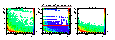
\includegraphics[width=\textwidth]{pictures/cross_section/eff_err/eff_err_16375.pdf}
\caption{\small Distributions of the relative efficiency uncertainty versus efficiency (a) taking into account the weights (see Eq.~\eqref{eq:eff_err_weighted}) and (b) ignoring them (see Eq.~\eqref{eq:eff_err_unweighted}). The cut that aims to select the cells with reliable efficiency is shown by the red horizontal line in panel (b).  Panel (c) shows the influence of this cut on the distribution $\delta \mathcal{E}/\mathcal{E}$ (with the weights taken into account). The distributions are provided for one particular $\Delta W \Delta Q^2$ bin (with the central values specified in figure), and the color code represents the number of multi-dimensional cells within this bin. Note that the $z$-axis maximum for the plot (a) is set the same as for the plot (c).} \label{fig:eff_err}
\end{center}
\end{figure}


The number of reconstructed events in the revealed cells with unreliable efficiency is set to zero ($N_{rec} = 0$). Then such a cell is ranked as an ``empty cell" and, along with other empty cells, is subject to the filling procedure, which is described in Sect.~\ref{Sect:empt_cells}. 


The described above cut on the relative efficiency uncertainty directly impacts the cross section's uncertainties. On the one hand, it eliminates the $\Delta^{5} \tau$ bins with high relative efficiency uncertainty, thus reducing the total statistical uncertainty of the extracted cross sections (see Sect.~\ref{Sect:stat_uncert}). On the other hand, this cut increases the amount of empty cells, thus increasing the cross section's model dependence and the uncertainty associated with it (see Sect.~\ref{Sect:mod_dep}). The cut value is therefore chosen as a compromise between these two effects. 


The idea of this cut is taken from the study~\cite{Fed_an_note:2017,Fed_paper_2018}, which uses unweighted Monte Carlo simulation and therefore employs Eq.~\eqref{eq:eff_err_unweighted} to calculate the efficiency uncertainty. The study~\cite{Fed_an_note:2017,Fed_paper_2018} observed the similar cell clustering along horizontal stripes as that revealed in this analysis in the distributions of $\delta \widetilde{\mathcal{E}}/\widetilde{\mathcal{E}}$ versus $\widetilde{\mathcal{E}}$ (produced ignoring the weights) and also set the cut at the position of 0.3. 
%Therefore, in this analysis the cut position is chosen to be the same as in the study~\cite{Fed_an_note:2017,Fed_paper_2018} (i.e. at 0.3).


Note that in this particular analysis the formula~\eqref{eq:eff_err_unweighted} for the unweighted Monte Carlo is used only for selecting the bins with reliable efficiency, since it allows the pure statistical behavior of the efficiency uncertainty to be determined. For the estimation of the cross section's statistical uncertainty the weights are taken into account and the formula~\eqref{eq:eff_err_weighted} is applied (see Sect.~\ref{Sect:stat_uncert}).


 
